\documentclass[dvipdfmx,a4j]{jarticle}
\pagestyle{empty}
\usepackage{tikz}
\usetikzlibrary{shapes,calc}
\begin{document}
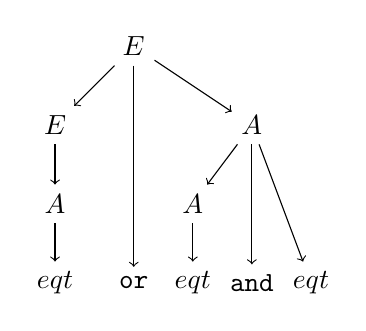
\begin{tikzpicture}
\node (N0) at (0,0) {$E$};
\node (N1) at (-1,-1) {$E$};
\node (N11) at (-1,-2) {$A$};
\node (N2) at (1.5,-1) {$A$};
\node (N3) at (0.75,-2) {$A$};

\node (N5) at (-1,-3) {$eqt$};
\node (N6) at (0,-3) {$\mathtt{or}$};
\node (N7) at (0.75,-3) {$eqt$};
\node (N8) at (1.5,-3) {$\mathtt{and}$};
\node (N9) at (2.25,-3) {$eqt$};

\path[->] (N0) edge (N1) (N0) edge (N2);
\path[->] (N1) edge (N11) (N11) edge (N5) (N2) edge (N3) (N2) edge (N9);
\path[->] (N0) edge (N6) (N3) edge (N7) (N2) edge (N8);
\end{tikzpicture}
\end{document}